% Pragmatic Intent: FR-12 paper draft (NeurIPS 2026 style, preprint mode).
% Every number in a table, and every number in the results prose, comes from paper/generated/,
% which src/analysis/paper_tables.py writes from the frozen test analysis. Do not type results by
% hand: change the analysis, regenerate, rebuild. See paper/README.md.
\documentclass{article}

\usepackage[preprint]{neurips_2026}

\usepackage[utf8]{inputenc}
\usepackage[T1]{fontenc}
\usepackage{hyperref}
\usepackage{url}
\usepackage{booktabs}
\usepackage{amsfonts}
\usepackage{amsmath}
\usepackage{nicefrac}
\usepackage{microtype}
\usepackage{xcolor}
\usepackage{graphicx}

% Generated; do not edit. Regenerate with:
%   python -m src.analysis.paper_tables --tables results/analysis/test --out paper/generated
% Source: results/analysis/test/h1_rates.csv sha256=28f332c7dd5086b37ad31e4148700eedf9fddf48d5b86959ee66b78598e02caa
% Source: results/analysis/test/h2_benefits.csv sha256=e99f198dc73e4bdbb85a55b98d0f462a1fc6feb482cf31b7bfba642217167382
% Source: results/analysis/test/mismatch_controls.csv sha256=8588c0a2b867e17ddf18e136c9320de0c7f9e1a59a10aa5044e7c53b4cf79994
% Source: results/analysis/test/primary_test.csv sha256=d056e1f1f4c5ae21ba2adc7f3829d4eceeb1130fa822ba711363464ab0f8f1e6
% Source: results/analysis/test/holm.csv sha256=ced3a28a8575314aad5009be2f278c8ad36f6e03aa7da3f36e3c3004982801c0
% Source: results/analysis/test/h4_rates.csv sha256=c403099cab74b7202dffd1f89b12cca5fc5db1f6a7d4cad3155ccebd1438bf22
% Source: results/analysis/test/sensitivity.csv sha256=6033a7e3d5aa02d6047298e97f6bd966d1354bf090990699d889160ebd4c9946
% Source: results/analysis/test/transfer.csv sha256=d1a7937896bd325c89a77037b3b55cc010d11692d7afa579c51b8cb252546639
% Analysis config: 231365295e22
\newcommand{\AnalysisConfig}{231365295e22}
\newcommand{\PrimaryEst}{$-$0.005}
\newcommand{\PrimaryCI}{[$-$0.027, 0.018]}
\newcommand{\PrimaryP}{0.686}
\newcommand{\PrimaryExamples}{2{,}137}
\newcommand{\PrimaryDialogues}{797}
\newcommand{\QuadEst}{+0.019}
\newcommand{\HoneEst}{+0.033}
\newcommand{\HoneCI}{[0.012, 0.054]}
\newcommand{\HoneP}{0.008}
\newcommand{\HfourEst}{+0.024}
\newcommand{\HfourCI}{[$-$0.005, 0.055]}
\newcommand{\HfourP}{0.213}
\newcommand{\SensEst}{$-$0.003}
\newcommand{\SensCI}{[$-$0.025, 0.020]}
\newcommand{\CueFreeEst}{+0.055}
\newcommand{\CueFreeCI}{[0.046, 0.064]}
\newcommand{\LthreeGain}{+0.045}
\newcommand{\LthreeCI}{[0.011, 0.080]}
\newcommand{\LthreeExamples}{323}
\newcommand{\ControlEst}{+0.057}
\newcommand{\ControlCI}{[0.048, 0.066]}
\newcommand{\OracleFull}{0.181}
\newcommand{\DetectFull}{0.991}
\newcommand{\QwenDetNone}{0.668}
\newcommand{\QwenDetFull}{0.672}
\newcommand{\TransferN}{194}
\newcommand{\TransferRecall}{0.031}
\newcommand{\TransferValue}{0.608}
\newcommand{\TransferEndToEnd}{0.021}
\newcommand{\HybridInterpNone}{0.181}
\newcommand{\HybridInterpOne}{0.200}
\newcommand{\HybridInterpFull}{0.186}
\newcommand{\HybridInterpMismatched}{0.130}
\newcommand{\HybridInterpMismatchedOne}{0.153}
\newcommand{\OneNoneEst}{+0.019}
\newcommand{\OneNoneCI}{[0.012, 0.027]}
\newcommand{\FullNoneEst}{+0.005}
\newcommand{\FullNoneCI}{[$-$0.004, 0.014]}
\newcommand{\FullOneEst}{$-$0.014}
\newcommand{\FullOneCI}{[$-$0.023, $-$0.006]}


% An unresolved item the draft owner must fill in before submission.
\newcommand{\todo}[1]{\textcolor{red}{[TODO: #1]}}

\title{Does Dialogue Context Help More When Requests Are Less Direct?\\
A Preregistered Test on Task-Oriented Dialogue Rewrites}

\author{%
  Sandy Thomas\\
  \todo{affiliation}\\
}

\begin{document}

\maketitle

\begin{abstract}
Assistants must recover what a user wants even when the request is phrased indirectly. A common
intuition is that preceding dialogue matters most for exactly those turns. We test that intuition
with a frozen, preregistered protocol on MultiWOZ dialogues whose user turns were rewritten into
direct and indirect variants by the DIRECT corpus. Each example is assigned a rule-based
indirectness level (L0--L3) and scored under five context conditions: none, the preceding turn,
the full history, and two mismatched histories taken from another dialogue. We evaluate request
detection and structured request interpretation for TF-IDF, DeBERTa-v3, Qwen2.5-7B-Instruct and a
routed hybrid. The confirmatory test, whether the full-history benefit grows from L0 to L2 for the
hybrid, is null: the linear contrast is \PrimaryEst{} with 95\% CI \PrimaryCI{} ($p=\PrimaryP$).
Context is nonetheless used: interpretation is \ControlEst{} \ControlCI{} higher with the true
history than with another dialogue's. The main bottleneck is not detection, which is near ceiling on gold
requests (\DetectFull), but interpretation, where even oracle routing reaches only \OracleFull.
Contrary to the usual expectation, interpretation success rises rather than falls from L0 to L2.
We release the code, frozen configuration and table-generation pipeline.
\end{abstract}

% ---------------------------------------------------------------------------------------------
\section{Introduction}
\label{sec:intro}

Users rarely state requests in the form an assistant is trained to parse. ``I need a cheap hotel
in the north'' and ``The north would be handy, and money's a bit tight this month'' can ask for
the same thing. The second leaves the request implicit and relies on the listener to recover it,
often with help from what was said earlier \citep{searle1975indirect,blumkulka1989ccsarp}. For a
task-oriented assistant this raises two practical questions. Does the system notice that a
request was made (\emph{detection})? And does it recover what was asked for, the intent and its
slot values (\emph{interpretation})?

A natural hypothesis is that dialogue context helps more as requests become less direct: a direct
request carries its own content, whereas a hint needs the conversation to be understood. This
paper tests that hypothesis (H2) under a protocol that was frozen before any test-set result was
seen. We also report three secondary questions fixed in the same protocol: whether performance
falls as indirectness increases (H1), whether the context benefit differs by model family (H3),
and whether detection degrades more slowly than interpretation (H4).

Our setting holds the target wording fixed and varies only the context. We use DIRECT
\citep{takayama2021direct}, which rewrites MultiWOZ \citep{budzianowski2018multiwoz,eric2020multiwoz21}
user turns into direct and indirect paraphrases, and assign each rewrite a level with a versioned
wording rule. Every example is then scored under five context conditions, including two
\emph{mismatched} conditions that substitute another dialogue's history as a control for models
that merely benefit from extra text.

\paragraph{Findings.}
\begin{itemize}
  \item The preregistered interaction is null. For the routed hybrid, the L2$-$L0 difference in
        the full-history benefit is \PrimaryEst{} \PrimaryCI{} on \PrimaryExamples{} L2 examples
        from \PrimaryDialogues{} dialogues. Overall, full history adds only \FullNoneEst{}
        \FullNoneCI{} to interpretation; the single preceding turn adds \OneNoneEst{} \OneNoneCI.
  \item Models do use context. The true history beats another dialogue's history by
        \ControlEst{} \ControlCI{} in interpretation, and the effect survives removing donors that
        mention a cue (\CueFreeEst{} \CueFreeCI).
  \item Interpretation, not detection, is the bottleneck. On gold indirect requests the hybrid
        detects \DetectFull{} under full context, yet oracle interpretation is \OracleFull, and
        routed interpretation matches it.
  \item H1 is reversed for interpretation: success rises from L0 to L2 by \HoneEst{} \HoneCI{}
        (Holm $p=\HoneP$). Detection falls slightly over the same range.
  \item Intent matters more than level (exploratory). The full-history benefit runs from
        \IntentBookingEst{} for booking to \IntentRecommendationEst{} for recommendation, and
        info-seeking requests are almost never interpreted exactly.
\end{itemize}

We make no claim to be first with a context ablation, a graded notion of indirectness or a
shuffled-context control; each has precedents (\S\ref{sec:related}). The contribution is a
controlled, preregistered combination of them for assistant requests, with detection, oracle
interpretation and routed interpretation scored on the same items.

% ---------------------------------------------------------------------------------------------
\section{Related work}
\label{sec:related}

\paragraph{Pragmatic meaning and assistant dialogue.}
Resources for pragmatic inference target different kinds of meaning. \citet{george2020implicatures}
annotate implied meanings in dialogue snippets, and Circa \citep{louis2020circa} covers indirect
answers to polar questions. Both support contextual interpretation, but neither labels requests
to an assistant. DIRECT \citep{takayama2021direct} is our closest predecessor: it augments
MultiWOZ with crowd-written pragmatic paraphrases and evaluates directness prediction and
paraphrase generation with and without dialogue history, finding that history does not help every
task. That mixed result motivates scoring detection and interpretation separately. We keep DIRECT's
rewrites but replace its variant labels with rule-assigned wording levels. IndirectRequests
\citep{mannekote2025indirect} instead generates requests from SGD schemas with an LLM and has them
rated by crowd workers. We use it only as a separately reported transfer test.

\paragraph{Context, indirectness and evaluation design.}
Context-dependent speech-act interpretation has a long experimental lineage, from indirect
speech-act schemas \citep{roque2020isa} to INDIR-IT's paired literal and indirect contexts
\citep{orsini2025indirit}. DRInQ \citep{arai2026drinq} varies the context around fixed questions,
and READI \citep{kim2026readi} grades indirectness in a visual setting with a shuffled-image
control. Neither contextual inference nor a corrupted-context control is new here. Broader
conversational context also helps dialogue-act recognition \citep{zelasko2021dialogacts}, and
lexical classifiers with and without context \citep{li2022implicatures} show why a context-blind
baseline is informative. Wider evaluations compare human and model pragmatic interpretation
\citep{hu2023pragmatics}, and \citet{ma2025survey} survey the area. Our narrower question is
whether the benefit of the preceding \emph{text} context varies across indirectness levels in
assistant dialogue, with the target wording and the reference acts held fixed across conditions.

% ---------------------------------------------------------------------------------------------
\section{Data and annotation}
\label{sec:data}

\paragraph{Source and splits.}
We join DIRECT's rewrites to MultiWOZ~2.1 and keep MultiWOZ's official splits; DIRECT training
dialogues that MultiWOZ assigns to validation become development data. Each example is one
rewritten user turn after the first turn, so every example has some history. A split audit,
completed before scoring, removed cross-split duplicates and inspected dialogues. The test set
holds 10{,}465 examples from 934 dialogues.\footnote{Counts from
\texttt{results/analysis/test/report.json} and the split-audit summary; see
Appendix~\ref{app:repro}.} Exact duplicates within test are flagged (15.0\%) and re-analysed in a
sensitivity line that drops them.

\paragraph{Labels.}
The reference for each example is the original turn's MultiWOZ dialogue acts. These map to a
request type (direct, indirect or no request) and, for requests, to an intent category
(\texttt{cat-v1}: information seeking, booking, travel, recommendation) with its slot values.
DIRECT's variant label supplies the direct/indirect distinction for Stage~1.

\paragraph{Indirectness levels.}
A versioned rule set (\texttt{auto-v1}) assigns each rewrite one level, applied in order:
\textbf{NR} (only social acts), \textbf{L0} (a need or want statement, a command or a plain
question), \textbf{L1} (a conventional formula such as ``could you''), \textbf{NR} (declining an
offer), \textbf{INF} (no preference, a bare yes/no or a fragment), \textbf{L2} (a hint that names
the detail sought), and \textbf{L3} (anything else). The levels are a proxy, not gold. Checked
against the author's labels, the rules agreed on 31 of 39 items ($\kappa=0.74$) in two rounds and
29 of 30 ($\kappa=0.93$) in a third. L3 is the weakest level: only 12 of 40 audited L3 items were
truly L3, most of the rest being non-requests or L2. The rules also show that DIRECT's ``indirect''
label is weak for our purpose: about 27\% of indirect test rewrites read as plain L0 requests.

\paragraph{Context conditions.}
The target text is identical in all five conditions. \texttt{none} gives the target alone,
\texttt{one} adds the single preceding turn, and \texttt{full} adds every preceding turn.
\texttt{mismatched} and \texttt{mismatched\_one} substitute the history of a donor dialogue from
the same split, chosen by a seeded draw from dialogues sharing no domain with the target.
Turns are rendered as \texttt{User:}/\texttt{System:} lines. Context plus target is capped at 350
whitespace tokens by dropping the oldest turns, which affects 0.9\% of test examples. Contrasts
with a mismatched condition use the 10{,}393 examples that have a donor.

% ---------------------------------------------------------------------------------------------
\section{Task and models}
\label{sec:models}

\paragraph{Two stages.}
Stage~1 classifies a turn as a direct request, an indirect request or no request. Stage~2
interprets a request as one \texttt{cat-v1} category plus slot--value pairs under a closed schema
(56 slot keys). Our primary endpoint, \emph{request interpretation}, counts an example as correct
when it is a gold request, the system predicts some request, and the category and normalised slot
values match exactly. Invalid model output counts as an error. \emph{Detection} below means
three-way Stage~1 accuracy over all examples, unless stated otherwise.

\paragraph{Systems.}
\begin{itemize}
  \item \textbf{TF-IDF} logistic regression on word $n$-grams ($n\le2$) \citep{pedregosa2011sklearn},
        trained once on \texttt{full} inputs: an \emph{utterance} variant that never sees
        context, whose benefit is zero by construction, and a \emph{context} variant.
  \item \textbf{DeBERTa-v3-base and -large} \citep{he2023debertav3}, fine-tuned for Stage~1 with
        five seeds under each of \texttt{none}, \texttt{one} and \texttt{full}.
  \item \textbf{Qwen2.5-7B-Instruct} \citep{qwen2024qwen25}, prompted for both stages with six
        fixed DIRECT-train examples (prompt P2, chosen over a zero-shot prompt on development
        data), greedy decoding and schema-constrained output via vLLM \citep{kwon2023vllm}.
  \item \textbf{Routed hybrid} (the primary system): the DeBERTa-v3-large detector routes each
        turn, and Qwen interprets the turns routed as requests. A turn routed to no request stays
        a non-request.
\end{itemize}

\paragraph{Lines.}
A trained system can be scored two ways. On the \emph{matched} line, condition $c$ is scored by
the model trained on $c$; this is the primary line. On the \emph{test-time} line, the model
trained on \texttt{full} is scored under every condition. Untrained and single-model systems have
only the test-time line. Mismatched contrasts always use the test-time line.

% ---------------------------------------------------------------------------------------------
\section{Experimental setup}
\label{sec:setup}

\paragraph{Preregistration.}
The data, rules, prompts, model revisions, hyperparameters and analysis plan were frozen in a
hashed record before test inference. One amendment, logged before any test output was read,
re-pinned the selected prompt after a development-set bug fix. An earlier Qwen test run that
predated the amendment was archived unread.

\paragraph{Prompt selection.}
Two prompts were written before any development run: P1 gives zero-shot schema instructions,
and P2 adds six DIRECT-train examples drawn with a fixed seed. Each was run on every development
example under \texttt{none} and \texttt{full}. It was scored as the hybrid's request
interpretation, averaged over both conditions and the five router seeds, a metric that does not
favour either answer to H2. In a first round both prompts broke the preregistered 2\% limit on
invalid output (P1 2.23\%, P2 2.02\%), so both were fixed and rerun. In the second round P2
scored 0.177 against P1's 0.128, with 0.61\% and 0.94\% invalid output, and was
selected.\footnote{Development-set numbers from
\texttt{specs/009-llm-routed-hybrid/verification.md}; no test data was used.}

\paragraph{Training and inference.}
DeBERTa-v3-base and -large are fine-tuned as cross-encoders on the three-way Stage~1 label, with
an effective batch of 32, two epochs, weight decay 0.01, bf16 and inputs of at most 512 subword
tokens. Base uses a learning rate of $2\times10^{-5}$ with 6\% warmup; large uses
$1\times10^{-5}$ with 10\% warmup, because large DeBERTa can collapse to a single class at higher
rates. TF-IDF uses unigrams and bigrams with a minimum document frequency of 2 and $C=1$; its
context variant keeps separate vocabularies for the target turn and the history. Qwen runs at a
pinned model revision in vLLM, with temperature 0, at most 256 output tokens and a 4{,}096-token
window. Encoder runs used one NVIDIA RTX~5090; one DeBERTa-v3-large seed (three training
conditions) took about 2.3 hours. Exact values are in the frozen configuration files
(Appendix~\ref{app:repro}).

\paragraph{Hypotheses and tests.}
H2 is the single confirmatory test: for the hybrid on the matched line, the linear
$(-1,0,+1)$ contrast over L0, L1 and L2 of the \texttt{full}$-$\texttt{none} benefit in request
interpretation. L3, INF and NR are excluded from the trend because their rules are least
reliable. A secondary family of nine statistics is Holm-adjusted together
\citep{holm1979}: the H1 interpretation trend, the detection-only H2 trend, the H4 contrast,
the \texttt{full}$-$\texttt{mismatched} control, and five H3 differences between each panel
system's test-time context benefit and the hybrid's. H4 is the L0$-$L2 drop in detection minus
the drop in oracle interpretation under \texttt{full}, on gold indirect requests, with the
protocol predicting a negative value. Everything else is descriptive.

\paragraph{Statistics.}
All intervals are 95\% percentile intervals from a dialogue-cluster bootstrap with 10{,}000
replicates \citep{efron1993bootstrap}, resampling dialogues because turns from one dialogue are
dependent. Seeds are averaged per example before resampling. A level cell with fewer than 30
dialogues is marked sparse and never tested.

% ---------------------------------------------------------------------------------------------
\section{Results}
\label{sec:results}

\begin{table}[t]
  \caption{Overall success by context condition on test. Detection is three-way Stage~1
  accuracy over all examples; interp.\ is request interpretation on gold requests. DeBERTa and
  the hybrid are on the matched line; TF-IDF and Qwen have one model each (test-time line). The
  last column is the test-time \texttt{full}$-$\texttt{mismatched} control.}
  \label{tab:overall}
  \centering
  \small
  % Generated; do not edit. Regenerate with:
%   python -m src.analysis.paper_tables --tables results/analysis/test --out paper/generated
% Source: results/analysis/test/h1_rates.csv sha256=28f332c7dd5086b37ad31e4148700eedf9fddf48d5b86959ee66b78598e02caa
% Source: results/analysis/test/mismatch_controls.csv sha256=8588c0a2b867e17ddf18e136c9320de0c7f9e1a59a10aa5044e7c53b4cf79994
% Analysis config: 231365295e22
\begin{tabular}{llrrrrrr}
\toprule
System & Endpoint & none & one & full & mism. & mism.-one & full$-$mism. \\
\midrule
TF-IDF (utterance) & detection & 0.897 & 0.897 & 0.897 & 0.897 & 0.897 & 0.000 \\
TF-IDF (context) & detection & 0.885 & 0.891 & 0.895 & 0.889 & 0.885 & +0.006 \\
DeBERTa-v3-base & detection & 0.924 & 0.926 & 0.926 & 0.911 & 0.910 & +0.015 \\
DeBERTa-v3-large & detection & 0.927 & 0.930 & 0.928 & 0.903 & 0.905 & +0.025 \\
Qwen2.5-7B-Instruct & detection & 0.668 & 0.678 & 0.672 & 0.598 & 0.622 & +0.073 \\
Routed hybrid & detection & 0.921 & 0.927 & 0.926 & 0.892 & 0.895 & +0.034 \\
\midrule
Qwen2.5-7B-Instruct & interp. & 0.179 & 0.197 & 0.186 & 0.127 & 0.148 & +0.059 \\
Routed hybrid & interp. & 0.181 & 0.200 & 0.186 & 0.130 & 0.153 & +0.057 \\
\bottomrule
\end{tabular}

\end{table}

\paragraph{Overall.}
Table~\ref{tab:overall} gives each system's success under every condition. The fine-tuned
detectors reach about 0.93 three-way accuracy whatever the context, and Qwen's prompted detection
is much weaker (\QwenDetNone{} without context). Interpretation is low for every system: the hybrid
reaches \HybridInterpNone{} without context, \HybridInterpOne{} with one turn and
\HybridInterpFull{} with the full history. The single preceding turn helps most
(\OneNoneEst{} \OneNoneCI{} over none), and adding the rest of the history takes some of that
back (\FullOneEst{} \FullOneCI).

\begin{table}[t]
  \caption{The preregistered test and the Holm-adjusted secondary family. Contrasts are
  L2$-$L0 linear trends unless named otherwise; H3 rows compare each system's test-time
  \texttt{full}$-$\texttt{none} benefit with the hybrid's on the named endpoint.}
  \label{tab:confirmatory}
  \centering
  \small
  % Generated; do not edit. Regenerate with:
%   python -m src.analysis.paper_tables --tables results/analysis/test --out paper/generated
% Source: results/analysis/test/primary_test.csv sha256=d056e1f1f4c5ae21ba2adc7f3829d4eceeb1130fa822ba711363464ab0f8f1e6
% Source: results/analysis/test/holm.csv sha256=ced3a28a8575314aad5009be2f278c8ad36f6e03aa7da3f36e3c3004982801c0
% Analysis config: 231365295e22
\begin{tabular}{lrcr}
\toprule
Statistic & Estimate & 95\% CI & $p$ \\
\midrule
\multicolumn{4}{l}{\emph{Confirmatory (H2): routed hybrid, interpretation, L2$-$L0 of full$-$none}} \\
Linear contrast & $-$0.005 & [$-$0.027, 0.018] & 0.686 \\
Quadratic term (descriptive) & +0.019 & [$-$0.020, 0.057] & -- \\
\midrule
\multicolumn{4}{l}{\emph{Secondary family (Holm-adjusted $p$)}} \\
H1: interpretation trend L2$-$L0, none & +0.033 & [0.012, 0.054] & 0.008 \\
H2 (detection): L2$-$L0 of full$-$none & 0.000 & [$-$0.008, 0.009] & 0.940 \\
H4: detection drop $-$ oracle drop & +0.024 & [$-$0.005, 0.055] & 0.213 \\
Control: full$-$mismatched (interp.) & +0.057 & [0.048, 0.066] & $<$0.001 \\
H3: TF-IDF (utterance) $-$ hybrid (detection) & $-$0.089 & [$-$0.093, $-$0.084] & $<$0.001 \\
H3: TF-IDF (context) $-$ hybrid (detection) & $-$0.079 & [$-$0.084, $-$0.073] & $<$0.001 \\
H3: DeBERTa-v3-base $-$ hybrid (detection) & $-$0.071 & [$-$0.075, $-$0.067] & $<$0.001 \\
H3: DeBERTa-v3-large $-$ hybrid (detection) & $-$0.004 & [$-$0.006, $-$0.002] & $<$0.001 \\
H3: Qwen2.5-7B-Instruct $-$ hybrid (interp.) & +0.002 & [0.001, 0.003] & 0.004 \\
\bottomrule
\end{tabular}

\end{table}

\paragraph{H2: no interaction.}
The confirmatory contrast is \PrimaryEst{} \PrimaryCI{} ($p=\PrimaryP$; Table~\ref{tab:confirmatory}).
Dropping exact duplicates gives \SensEst{} \SensCI. The detection-only trend is also flat. Per
level (Table~\ref{tab:levels}), the full-history benefit is within $\pm0.01$ for L0--L2. The only
level with a clearly positive benefit is L3 (\LthreeGain{} \LthreeCI{}, $n=\LthreeExamples$),
which lies outside the prespecified trend and is the least reliable rule level, so we treat it as
exploratory.

\begin{table}[t]
  \caption{Routed hybrid by rule level (matched line). $n$ counts gold requests with a mapped
  category, so NR here holds the few gold requests the rules call non-requests. Detection is
  three-way Stage~1 accuracy on all examples at that level.}
  \label{tab:levels}
  \centering
  \small
  % Generated; do not edit. Regenerate with:
%   python -m src.analysis.paper_tables --tables results/analysis/test --out paper/generated
% Source: results/analysis/test/h1_rates.csv sha256=28f332c7dd5086b37ad31e4148700eedf9fddf48d5b86959ee66b78598e02caa
% Source: results/analysis/test/h2_benefits.csv sha256=e99f198dc73e4bdbb85a55b98d0f462a1fc6feb482cf31b7bfba642217167382
% Analysis config: 231365295e22
\begin{tabular}{lrrrcrr}
\toprule
Level & $n$ & interp.\ none & interp.\ full & full$-$none [95\% CI] & detect.\ none & detect.\ full \\
\midrule
L0 & 3843 & 0.171 & 0.179 & +0.008 [$-$0.004, 0.020] & 0.915 & 0.920 \\
L1 & 1759 & 0.193 & 0.190 & $-$0.003 [$-$0.020, 0.014] & 0.936 & 0.941 \\
L2 & 2137 & 0.204 & 0.207 & +0.003 [$-$0.016, 0.023] & 0.891 & 0.897 \\
L3 & 323 & 0.071 & 0.116 & +0.045 [0.011, 0.080] & 0.852 & 0.846 \\
INF & 178 & 0.169 & 0.180 & +0.011 [$-$0.041, 0.065] & 0.824 & 0.838 \\
NR & 77 & 0.273 & 0.156 & $-$0.117 [$-$0.216, $-$0.024] & 0.966 & 0.971 \\
\bottomrule
\end{tabular}

\end{table}

\paragraph{Context is used.}
A null interaction does not mean the models ignore context. Hybrid interpretation is
\ControlEst{} \ControlCI{} higher with the true history than with another dialogue's, and the control is positive
for every context-reading system in Table~\ref{tab:overall}. True history therefore carries
information the models use; its benefit over no history is small because the rewritten target
turn usually already states the category and slot values.

\paragraph{H1 reversed for interpretation.}
Interpretation success rises from L0 to L2 (\HoneEst{} \HoneCI{}, Holm $p=\HoneP$), the opposite
of H1. Detection falls slightly over the same range (Table~\ref{tab:levels}). One reading is that
L2 hints, by the rule's definition, name the detail being sought, while many L0 rewrites are
underspecified requests (``I need a hotel'') whose slot values lie in earlier turns. Indirectness
is observed rather than manipulated here, so this is a description of the corpus, not a causal
effect of wording.

\paragraph{H3: family differences reflect training.}
All five H3 differences are significant after Holm adjustment, but four of them say more about
the test-time line than about families. The detector trained on \texttt{full} loses accuracy
when evaluated without context, which inflates its test-time benefit; systems trained or prompted
without that dependence show smaller benefits. The design-matched comparison
(Table~\ref{tab:overall}) shows no family with a large context benefit, and Qwen and the hybrid
differ by only \(0.002\) because they share one interpreter.

\begin{table}[t]
  \caption{Detection, oracle and routed interpretation for the hybrid on identical gold indirect
  requests (matched line).}
  \label{tab:stages}
  \centering
  \small
  % Generated; do not edit. Regenerate with:
%   python -m src.analysis.paper_tables --tables results/analysis/test --out paper/generated
% Source: results/analysis/test/h4_rates.csv sha256=c403099cab74b7202dffd1f89b12cca5fc5db1f6a7d4cad3155ccebd1438bf22
% Analysis config: 231365295e22
\begin{tabular}{lrrrrr}
\toprule
Measure & none & one & full & mism. & mism.-one \\
\midrule
Detection (gold requests) & 0.983 & 0.990 & 0.991 & 0.974 & 0.979 \\
Oracle interpretation & 0.167 & 0.188 & 0.181 & 0.110 & 0.135 \\
Routed interpretation & 0.167 & 0.188 & 0.181 & 0.110 & 0.135 \\
\bottomrule
\end{tabular}

\end{table}

\paragraph{H4: interpretation is the bottleneck.}
On gold indirect requests the router detects \DetectFull{} under \texttt{full}, but interpretation
given a perfect router (oracle) is \OracleFull, and routed interpretation equals it
(Table~\ref{tab:stages}). Routing therefore costs almost nothing; nearly all loss is in recovering
the category and slots. The H4 contrast is \HfourEst{} \HfourCI{} (Holm $p=\HfourP$): detection
does not degrade measurably more slowly than interpretation.

\begin{table}[t]
  \caption{Routed hybrid request interpretation by intent category (H5, exploratory; matched
  line). $n$ counts gold requests in the category.}
  \label{tab:intents}
  \centering
  \small
  % Generated; do not edit. Regenerate with:
%   python -m src.analysis.paper_tables --tables results/analysis/test --out paper/generated
% Source: results/analysis/test/h5_rates.csv sha256=90e63922de43926f685e645057f3f210008259209b7bf5c665a28541b6af707d
% Source: results/analysis/test/h5_benefits.csv sha256=e7b3475dce004cd55d9fd2c3fc923dcd06780bc1887be8327a9b67c1a31d3490
% Analysis config: 231365295e22
\begin{tabular}{lrrrrc}
\toprule
Intent & $n$ & none & one & full & full$-$none [95\% CI] \\
\midrule
Info-seeking & 2391 & 0.018 & 0.059 & 0.025 & +0.008 [$-$0.001, 0.017] \\
Booking & 1279 & 0.231 & 0.179 & 0.172 & $-$0.059 [$-$0.087, $-$0.031] \\
Travel & 2006 & 0.267 & 0.310 & 0.263 & $-$0.003 [$-$0.027, 0.020] \\
Recommendation & 2641 & 0.239 & 0.254 & 0.279 & +0.040 [0.023, 0.056] \\
\bottomrule
\end{tabular}

\end{table}

\paragraph{H5 (exploratory): intents differ more than levels.}
Interpretation varies far more across intents than across levels (Table~\ref{tab:intents}).
Info-seeking requests are almost never interpreted exactly (\IntentInfoSeekingFull{} under
\texttt{full}), against \IntentBookingFull{} to \IntentRecommendationFull{} for the other three
intents. Context also cuts both ways. The full-history benefit is \IntentBookingEst{}
\IntentBookingCI{} for booking but \IntentRecommendationEst{} \IntentRecommendationCI{} for
recommendation, and the two largely cancel in the overall benefit. Level and intent are
correlated, so we reweight each level's benefit to the pooled intent mix over L0--L2. The
standardized trend is \StdTrendEst{} \StdTrendCI, so the null interaction is not an artefact of
intent composition. One hypothesis for the booking loss, which the error audit
(\S\ref{sec:audit}) can test, is that the history offers slot values from earlier turns that are
absent from the target turn's reference, so copying them counts as an unsupported addition.

\begin{figure}[t]
  \centering
  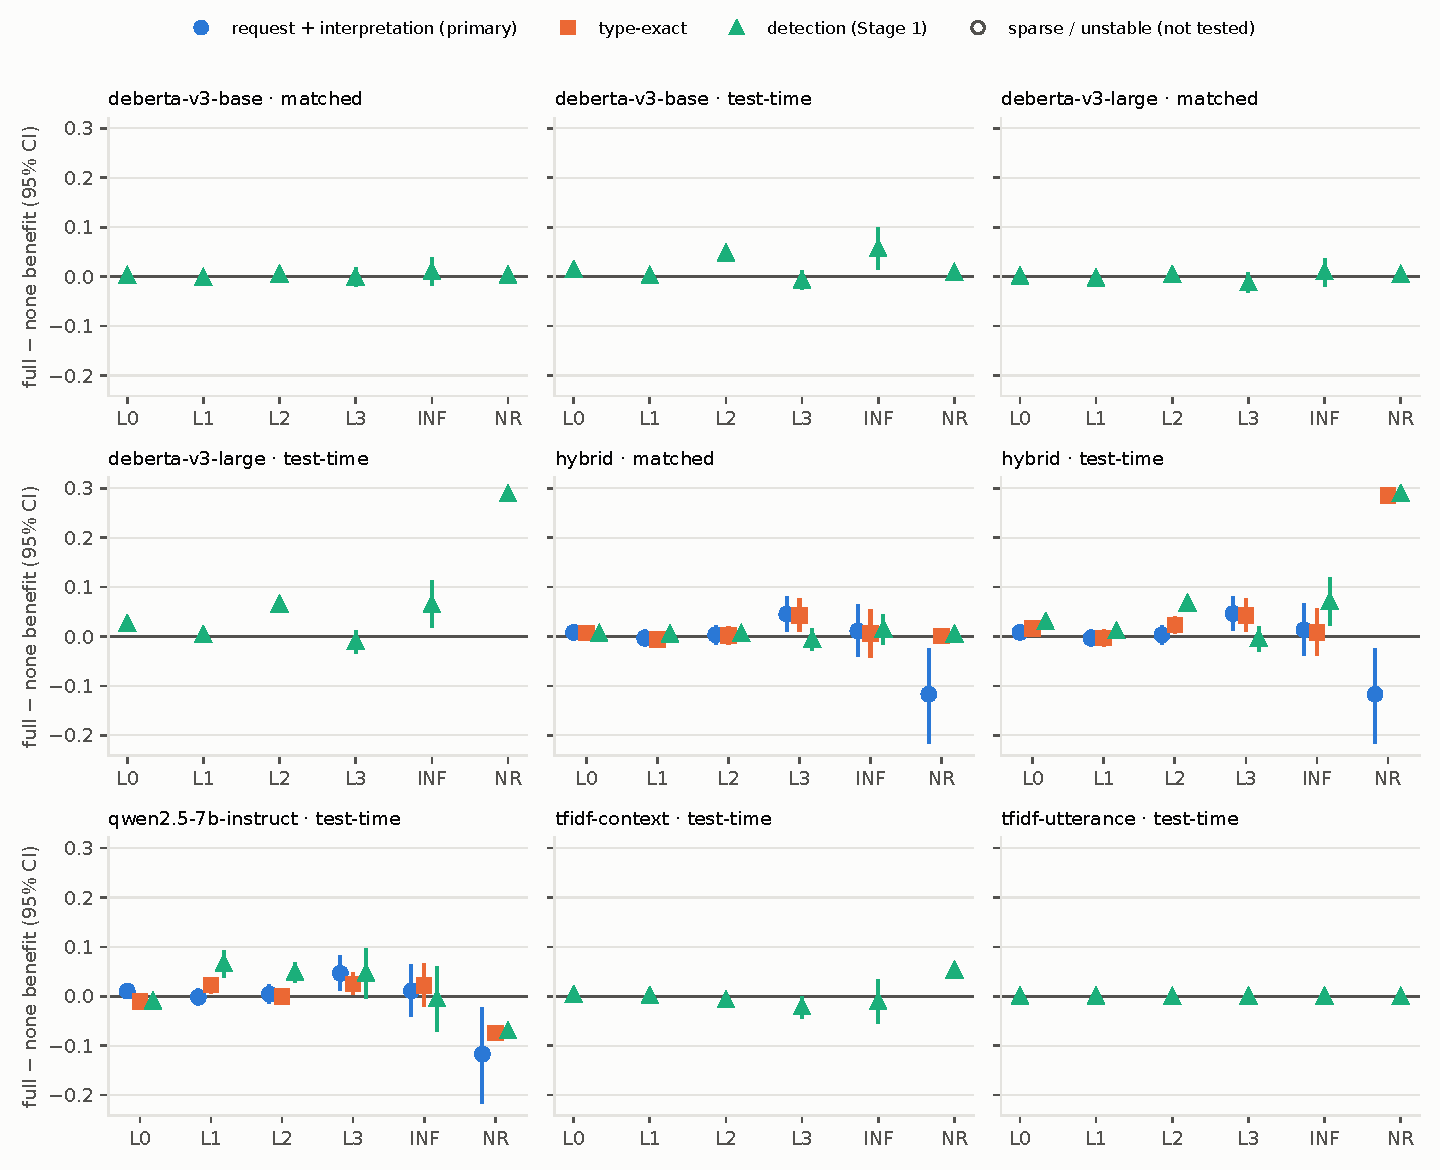
\includegraphics[width=\linewidth]{figures/context_by_level}
  \caption{\texttt{full}$-$\texttt{none} benefit by rule level, with 95\% dialogue-cluster
  bootstrap intervals, for every system and line. Hollow markers are sparse or unstable cells.}
  \label{fig:levels}
\end{figure}

Figure~\ref{fig:levels} shows the same per-level benefits for every system and line. Matched-line
benefits are near zero at every level, whereas the test-time detectors gain at NR and INF, where
the full-trained model has learned to rely on context.

\paragraph{Transfer.}
On the \TransferN{} IndirectRequests test items, run without context and zero-shot, Qwen recovers
requests poorly (recall \TransferRecall) although the values it returns are often right
(\TransferValue), for an end-to-end score of \TransferEndToEnd{} (Table~\ref{tab:transfer},
Appendix~\ref{app:extra}). This data is LLM-generated and its items have no non-requests, so it
cannot support a context claim or a false-positive rate.

% ---------------------------------------------------------------------------------------------
\section{Analysis and error audit}
\label{sec:audit}

\todo{Fill after the error audit. Design (fixed before scoring): 60 request-interpretation errors
of the hybrid under \texttt{full} on test, 15 per level L0--L3, drawn uniformly within each level
with a seeded draw. Each is coded once from a closed set: literal reading, wrong intent or slot,
missed cue, unsupported addition, source mismatch, malformed response, routing failure, with an
optional flag for a questionable reference. Report counts by level and code with the shortfall,
and the non-request false-positive rate, since over-inference is not sampled.}

% ---------------------------------------------------------------------------------------------
\section{Limitations}
\label{sec:limitations}

\textbf{Proxy labels.} The levels come from wording rules, not human judgments of indirectness,
and the L3 rule is unreliable. DIRECT's direct/indirect labels are weak, and the intent
reference is the original turn's acts, which a rewrite may not fully preserve. \textbf{One
annotator.} All rule checks and the error audit are by the author, so no inter-annotator agreement
is available. \textbf{Coverage.} \texttt{cat-v1} covers four MultiWOZ intents; troubleshooting,
advice and device control are absent. \textbf{Observational levels.} Levels are not randomised,
and they correlate with intent and turn position. \textbf{Panel.} One LLM and one interpreter
are tested, and the hybrid's five seeds share one interpreter pass, so its seed variation reflects
only the router. DeBERTa-v3-large's test-time line is seed-unstable without context.
\textbf{Inspected data.} Some test dialogues were inspected during development; they are
excluded as targets but stay in the donor pool, so 568 test examples take a mismatched history
from an inspected dialogue (split-audit summary in \texttt{data/manifests/}). \textbf{Context
format.} A 350-token budget truncates 0.9\% of histories, and only text context is studied.

% ---------------------------------------------------------------------------------------------
\section{Ethics and broader impact}
\label{sec:ethics}

The study uses public English corpora of simulated travel-booking dialogue with no personal data;
no new human-subject data was collected. Better recovery of indirect requests could make
assistants easier to use for people who prefer indirect phrasing, but over-inference, acting on a
request the user did not make, is a real risk, which is why we report non-request accuracy
alongside interpretation. LLM outputs may vary across runtimes even under greedy decoding; we
release all predictions. An AI coding assistant (Claude) wrote most of the analysis code under the
author's direction and review; all design decisions, labels and claims are the author's.

% ---------------------------------------------------------------------------------------------
\section{Conclusion}
\label{sec:conclusion}

Under a preregistered test, dialogue context did not help more as DIRECT rewrites became less
direct. Models do read the context, since a mismatched history hurts, but on these data the
target turn usually carries what is needed, and the hard part is recovering the exact category and
slots rather than noticing the request. Future work should test levels with independent human
judgments, deliberately underspecified targets, and more than one interpreter.

\begin{ack}
\todo{acknowledgements and funding, or remove.}
\end{ack}

\bibliographystyle{plainnat}
\bibliography{references}

% ---------------------------------------------------------------------------------------------
\appendix

\section{Reproduction and provenance}
\label{app:repro}

Every table is generated from the frozen test analysis (analysis config \texttt{\AnalysisConfig})
by a single command run from the repository root:
{\footnotesize
\begin{verbatim}
python -m src.analysis.paper_tables --tables results/analysis/test --out paper/generated
\end{verbatim}
}
Each generated fragment records the command, the SHA-256 of every input file and the analysis
config hash in its header comment. Table~\ref{tab:provenance} lists the inputs. The figure is drawn
from \texttt{results/analysis/test/figure\_data.csv} by \texttt{python -m src.analysis.figures} (matplotlib, via the \texttt{figures} uv group).
The freeze record, prompts, model revisions and per-run commands are in the repository's
\texttt{data/manifests/} and \texttt{configs/} directories: \texttt{configs/stage1/} for TF-IDF and DeBERTa,
\texttt{configs/llm/} for Qwen and its prompts.

\begin{table}[h]
  \caption{Inputs behind each generated fragment.}
  \label{tab:provenance}
  \centering
  \footnotesize
  % Generated; do not edit.
\begin{tabular}{lp{10cm}}
\toprule
Fragment & Sources under \texttt{results/analysis/test} (SHA-256 prefix) \\
\midrule
\texttt{overall.tex} & \texttt{h1\_rates.csv} (28f332c7dd50); \texttt{mismatch\_controls.csv} (8588c0a2b867) \\
\texttt{confirmatory.tex} & \texttt{primary\_test.csv} (d056e1f1f4c5); \texttt{holm.csv} (ced3a28a8575) \\
\texttt{levels.tex} & \texttt{h1\_rates.csv} (28f332c7dd50); \texttt{h2\_benefits.csv} (e99f198dc73e) \\
\texttt{stages.tex} & \texttt{h4\_rates.csv} (c403099cab74) \\
\texttt{intents.tex} & \texttt{h5\_rates.csv} (90e63922de43); \texttt{h5\_benefits.csv} (e7b3475dce00) \\
\texttt{transfer.tex} & \texttt{transfer.csv} (d1a7937896bd) \\
\texttt{numbers.tex} & \texttt{h1\_rates.csv} (28f332c7dd50); \texttt{h2\_benefits.csv} (e99f198dc73e); \texttt{mismatch\_controls.csv} (8588c0a2b867); \texttt{primary\_test.csv} (d056e1f1f4c5); \texttt{holm.csv} (ced3a28a8575); \texttt{h4\_rates.csv} (c403099cab74); \texttt{sensitivity.csv} (6033a7e3d5aa); \texttt{transfer.csv} (d1a7937896bd); \texttt{h5\_rates.csv} (90e63922de43); \texttt{h5\_benefits.csv} (e7b3475dce00); \texttt{h5\_standardized.csv} (34b9faaf0736) \\
\bottomrule
\end{tabular}

\end{table}

\section{Additional results}
\label{app:extra}

\begin{table}[h]
  \caption{IndirectRequests transfer (LLM-generated data, no context, reported separately from
  the main test).}
  \label{tab:transfer}
  \centering
  \small
  % Generated; do not edit. Regenerate with:
%   python -m src.analysis.paper_tables --tables results/analysis/test --out paper/generated
% Source: results/analysis/test/transfer.csv sha256=d1a7937896bd325c89a77037b3b55cc010d11692d7afa579c51b8cb252546639
% Analysis config: not recorded
\begin{tabular}{lcrrrrr}
\toprule
System & GPT family & $n$ & Request recall & Value acc. & End to end & Invalid \\
\midrule
Qwen2.5-7B-Instruct & no & 194 & 0.031 & 0.608 & 0.021 & 0 \\
\bottomrule
\end{tabular}

\end{table}

\end{document}
